\chapter{Experimental analysis}\label{chap:03}
%-----------------------------------------------------------%
\section{Analysis strategy}

The goal is to understand and measure the differences in the
behaviour of matter and antimatter with data recorded by the Run 1 of the LHCb experiment.

For this purpose, the analysis performed here compares the rates for the decays $B^{+} \rightarrow h^{+} h^{+} h^{-}$ and its antiparticle equivalent $B^{-} \rightarrow h^{-} h^{-} h^{+}$, where $h^{\pm}$ is a pion $\pi^{\pm}$ or a kaon $K^{\pm}$. The $B^{+}$ meson is composed of a $\bar{b}$ quark and $u$ quark. The pion $\pi^{+}$ is composed of a $\bar{d}$ and $u$ quarks, the kaon $K^{+}$ of a $\bar{s}$ and $u$ quarks. The decays studied proceed through the weak force (via $W^{\pm}$ bosons), where the CP symmetry is known to be violated\footnote{The observation of CP violation requires interference between two decay routes to the same final state.}.

Therefore we studied \emph{global} and \emph{local} CP violation, comparing the number of $B^{+}$ meson with the number of its anti-particle $B^{-}$. Since the value of CP violation might vary in different kinematic regions, then we focused on \emph{local} CP violation, meaning only on those regions were it is maximally violated.

In this analysis, we focus in particular the decays  $B^{\pm} \rightarrow K^{\pm} K^{+} K^{-}$.

Practically, the following programmes and frameworks are used to perform the analysis:
\href{https://www.python.org/}{$\texttt{Python}$},
\href{https://jupyter.org/}{$\texttt{Jupyter}$},
\href{https://root.cern/}{$\texttt{Root}$} \cite{brun1997root}.

The data we have at our disposal are in the file format common to LHC experiments, with the extension $\texttt{.root}$. Often files of this type are called \href{https://root.cern/doc/master/md_tree_2ntuple_2v7_2doc_2README.html}{$\texttt{tuple}$}. In this project, there are three different tuples:

\begin{itemize}
    \item $\texttt{PhaseSpaceSimulation.root}$, contains simulated data for the decay $B^{\pm} \rightarrow K^{\pm} K^{+} K^{-}$;
    \item $\texttt{B2HHH\_MagnetUp.root}$, contains data recorded by the LHCb experiment in 2011 reconstructed with a decay $B^{\pm} \rightarrow h^{\pm} h^{+} h^{-}$ with \enquote{up} magnet polarity;
    \item $\texttt{B2HHH\_MagnetDown.root}$, contains data recorded by the LHCb experiment in 2011 reconstructed with a decay $B^{\pm} \rightarrow h^{\pm} h^{+} h^{-}$ with \enquote{down} magnet polarity.
\end{itemize}

We handle the three $\texttt{.root}$ dataset file in Python converting those in the format of a $\texttt{pandas.DataFrame}$ with the help of the Python package:
\href{https://pypi.org/project/root-pandas/}{$\texttt{root-pandas}$}.
%-----------------------------------------------------------%
\section{Data analysis}
%-----------------------------------------------------------%

% Kinematics of simulated data / Invariant mass of final states particles
\subsection{Simulated data}\label{sec:sim_data}

We import the simulated data $\texttt{.root}$ file as a $\texttt{pandas.DataFrame}$:

\begin{lstlisting}
sim_data = read_root('/data/PhaseSpaceSimulation.root')
\end{lstlisting}

The data contains information about \enquote{events} that were observed in the detector. An event refers to the particles produced when two proton bunches of the beams collided at the LHC.

The detector has been used to reconstruct tracks that may have
come from the kaons; in the $\texttt{pandas.DataFrame}$ we have access to the measured momenta (\autoref{fig:x_momentum}), charge, and likelihood of the tracks being kaons.

\begin{figure}[H]
    %\setkeys{Gin}{draft=false}
	\centering
	\fcolorbox{black}{white}{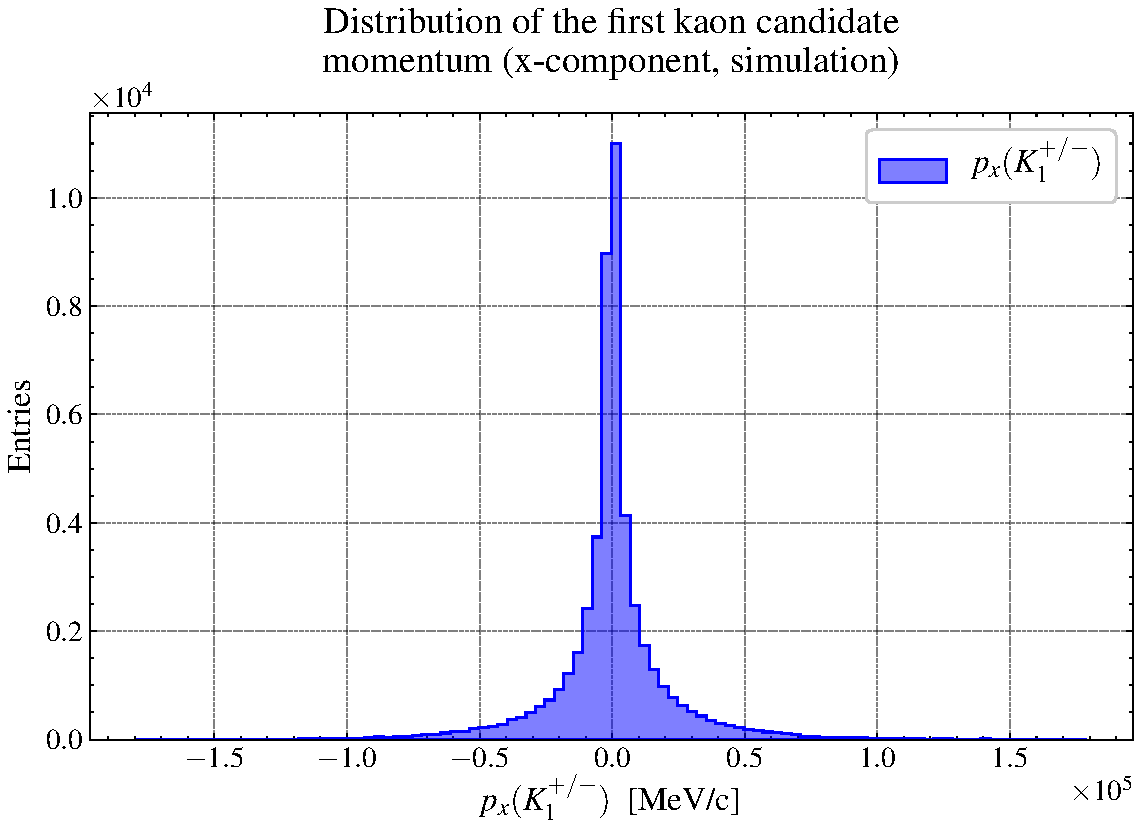
\includegraphics[scale=0.6]{graphs/H1_PX.pdf}}
	\caption{} %caption.}
	\label{fig:x_momentum}
\end{figure}

From the momentum for each axis of the three children particles we can compute the \emph{magnitude} of this quantity,
\begin{align}
   \norm {\underline{p}(K^i)} &= \sqrt{ p_{x}^2(K^i) + p_{y}^2(K^i) + p_{z}^2 (K^i)} \\ \notag\\
   \text{where} &\quad i \in \{1,2,3\}\text{.} \notag
\end{align}

that has the following distribution (\autoref{fig:mom_mag}),

\begin{figure}[H]
    %\setkeys{Gin}{draft=false}
	\centering
	\fcolorbox{black}{white}{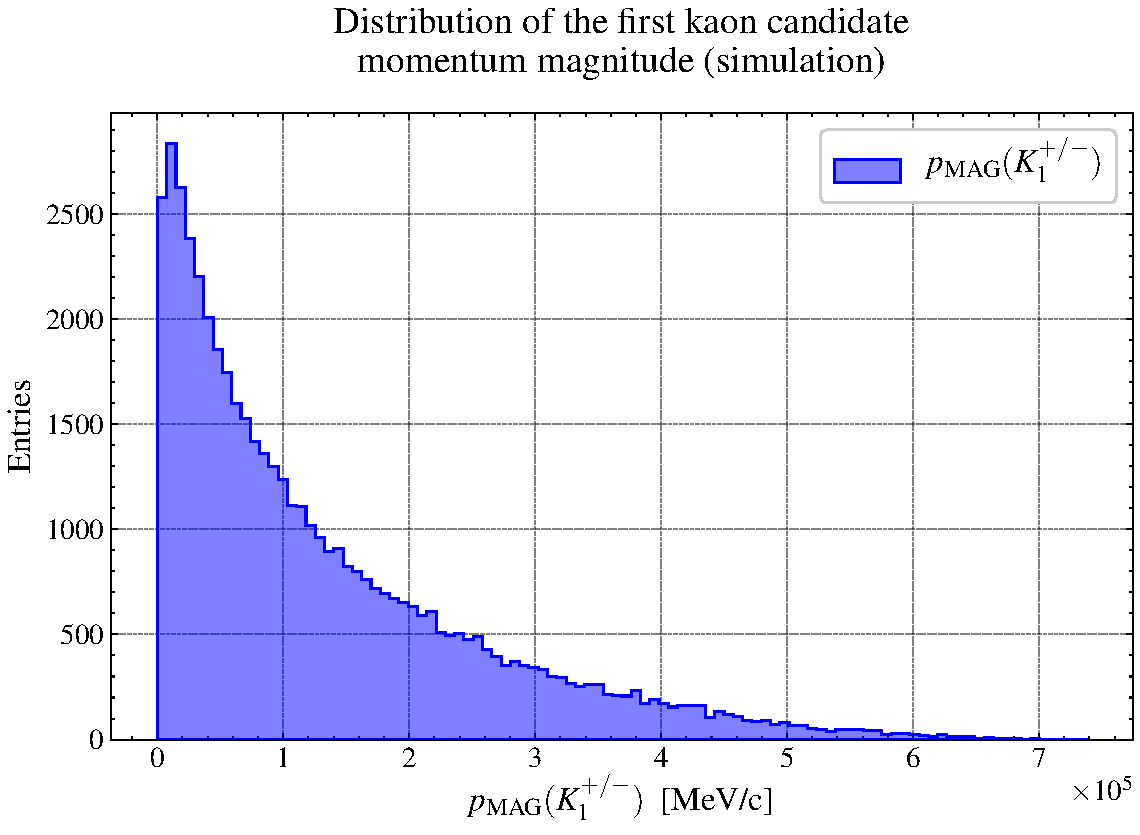
\includegraphics[scale=0.6]{graphs/H1_MAG.pdf}}
	\caption{} %caption.}
	\label{fig:mom_mag}
\end{figure}

The knowledge of the momentum magnitude with the kaon $K^{\pm}$ \href{https://pdglive.lbl.gov/Particle.action?node=S010&home=sumtabM}{mass} from the \href{https://pdglive.lbl.gov/Viewer.action}{PDG} \cite{PDG} allow us to compute the energy of the children particles from the \emph{energy–momentum relation}: $E^2 = p^2 +m^2$,

\begin{figure}[H]
    %\setkeys{Gin}{draft=false}
	\centering
	\fcolorbox{black}{white}{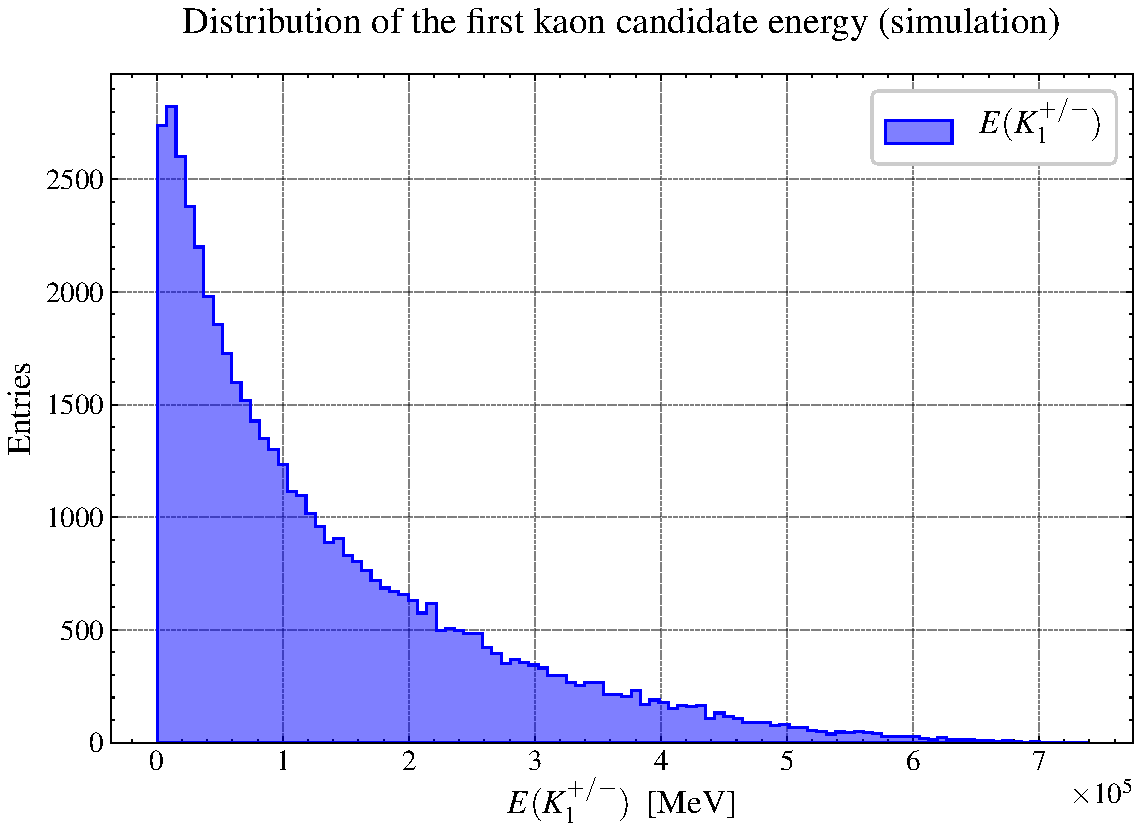
\includegraphics[scale=0.6]{graphs/H1_E.pdf}}
	\caption{} %caption.}
	%\label{fig:enter-label}
\end{figure}

Once computed the energy of the three kaons, taking advantage of the \emph{conservation of energy and momentum}, we can compute the energy and momentum of the mother particle $B^{\pm}$ as:

\begin{equation}
    E(B) = \sum_{i=1}^{3} E(K^{i})
\end{equation}
and
\begin{equation}
\hspace{1.2cm}
    \begin{dcases}
        p_x(B) = \sum_{i=1}^{3} p_x(K^{i}) \\
        p_y(B) = \sum_{i=1}^{3} p_y(K^{i}) \hspace{0.4cm}
        \Longrightarrow \hspace{0.4cm}
        \sqrt{ p_{x}^2(B) + p_{y}^2(B) + p_{z}^2(B) } = \norm {\underline{p}(B)} \\
        p_z(B) = \sum_{i=1}^{3} p_z(K^{i})
    \end{dcases}
\end{equation}
finally the $B^{\pm}$ invariant mass, resulting in the distribution of \autoref{fig:inv_mass_sim}

\begin{equation}
    m(B) = \sqrt{E^2(B)-p^2(B)}
\end{equation}

\begin{figure}[H]
    %\setkeys{Gin}{draft=false}
	\centering
	\fcolorbox{black}{white}{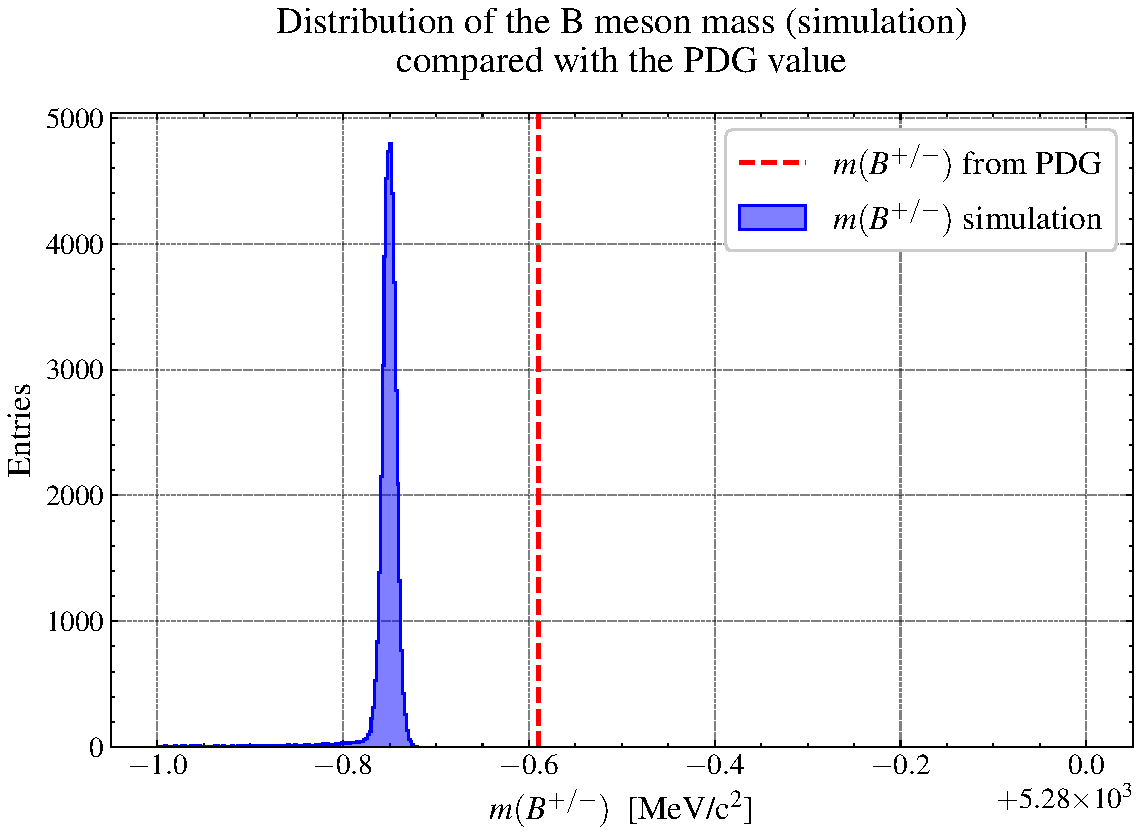
\includegraphics[scale=0.6]{graphs/B_M.pdf}}
	\caption{} %caption.}
	\label{fig:inv_mass_sim}
\end{figure}

%-----------------------------------------------------------%

% Preselection
\subsection{Real data}

The \emph{real data} have been pre-filtered to identify only events that are likely to come from $B^{\pm}$ mesons, decaying into three final state charged particles ($\mu$, $\pi^{\pm}$, $K^{\pm}$). We are interested only in the kaons final state, so we need to define a preselection over all the the possible children particles: in order to reduce the combinatorial background and the contribution of misidentified final state particles, the probability that the particles are pions ($\texttt{ProbPi}$) and the probability that the particle is a kaon ($\texttt{ProbK}$) have been determined for each of the three candidates.
In \autoref{fig:prob_pi} and \autoref{fig:prob_k} are shown the probability distributions of $h^{1}$.

\newpage
\begin{multicols}{2}
    \begin{figure}[H]
        %\setkeys{Gin}{draft=false}
    	\centering
    	\fcolorbox{black}{white}{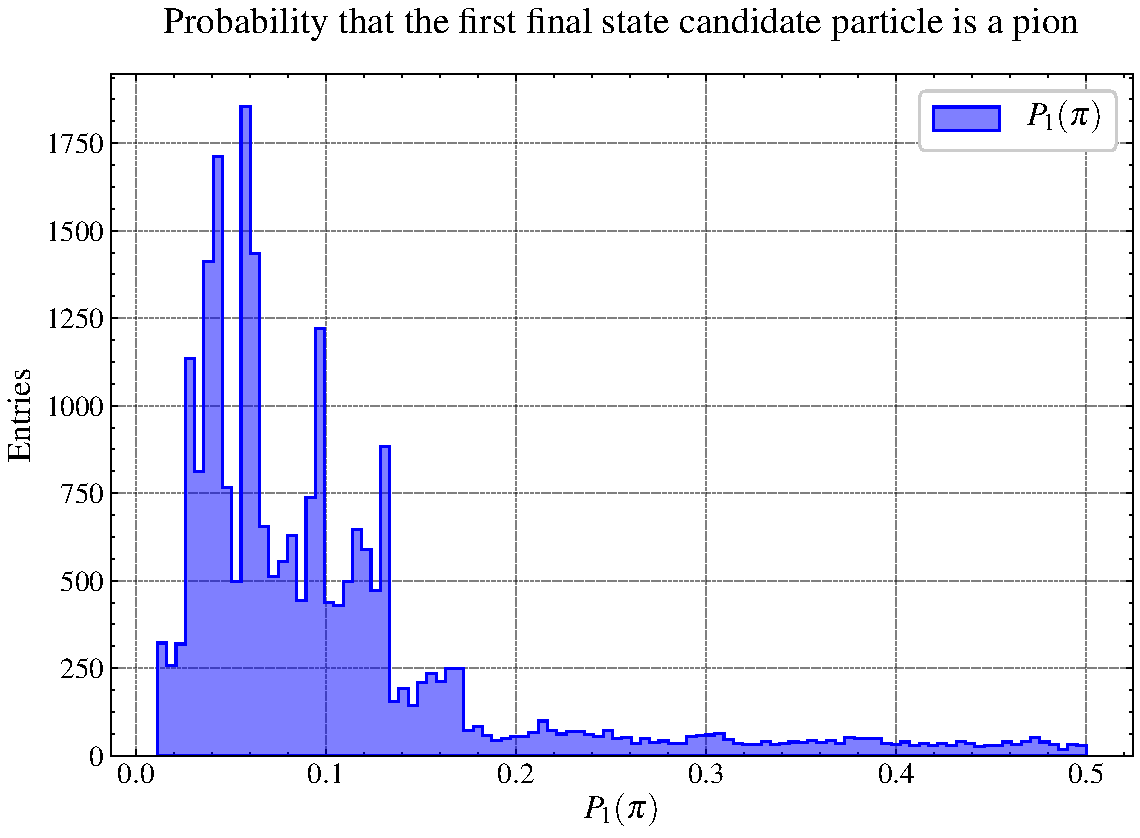
\includegraphics[scale=0.3]{graphs/H1_ProbPi.pdf}}
    	\caption{} %caption.}
    	\label{fig:prob_pi}
    \end{figure}

    \begin{figure}[H]
        %\setkeys{Gin}{draft=false}
    	\centering
    	\fcolorbox{black}{white}{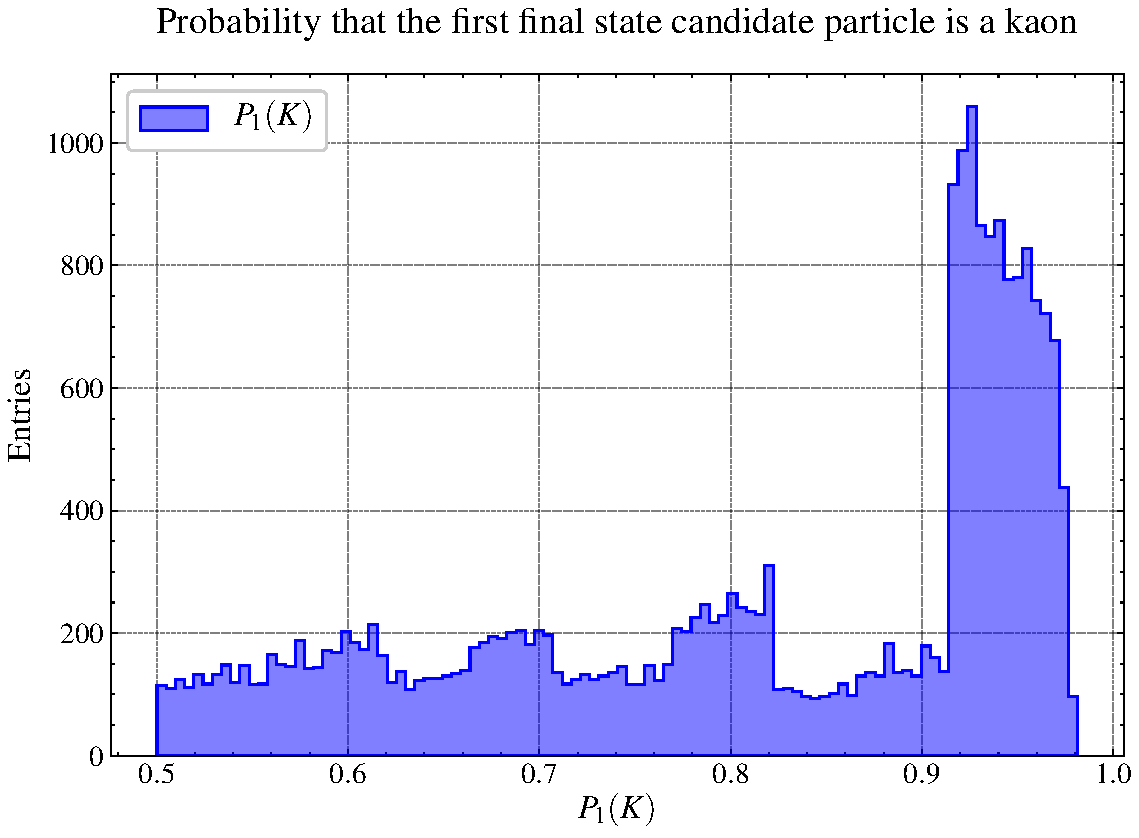
\includegraphics[scale=0.3]{graphs/H1_ProbK.pdf}}
    	\caption{} %caption.}
    	\label{fig:prob_k}
    \end{figure}
\end{multicols}

The preselection is, concretely, done using the following cuts on the real data:

\begin{center}
    \efbox{\begin{tabu}{|l|[1.2pt]c|c|c|}
        \hline
        \multicolumn{4}{|c|}{}\\
        \multicolumn{4}{|c|}{\textbf{\large Preselection}}\\
        \multicolumn{4}{|c|}{}\\
        \tabucline[1.2pt]{-}
        \multicolumn{1}{|c|[1.2pt]}{\textbf{Variable}} & $\bm{h^{1}}$ & $\bm{h^{2}}$ &
        \multicolumn{1}{c|}{$\bm{h^{3}}$}\\
        \tabucline[1.2pt]{-}
        $\texttt{isMuon}$ & not & not & not\\
        $\texttt{ProbPi}$ & $<0.5$ & $<0.5$ & $<0.5$\\
        $\texttt{ProbK}$ & $>0.5$ & $>0.5$ & $>0.5$\\
        \hline
    \end{tabu}}
\end{center}

Here, the preselection variable and the real data import from the Pyhton code,

\begin{lstlisting}
preselection = ('!H1_isMuon & H1_ProbPi<0.5 & H1_ProbK>0.5 & '+
                '!H2_isMuon & H2_ProbPi<0.5 & H2_ProbK>0.5 & '+
                '!H3_isMuon & H3_ProbPi<0.5 & H3_ProbK>0.5')

real_data = read_root(['/data/B2HHH_MagnetUp.root',
                       '/data/B2HHH_MagnetDown.root'],
                      where=preselection)
\end{lstlisting}

Once selected the \enquote{best} data for our purpose, we repeat the same procedure as in \Cref{sec:sim_data} to compute the $B^{\pm}$ invariant mass distribution for the real data (\autoref{fig:B_M_data}).

\begin{figure}[H]
    %\setkeys{Gin}{draft=false}
	\centering
	\fcolorbox{black}{white}{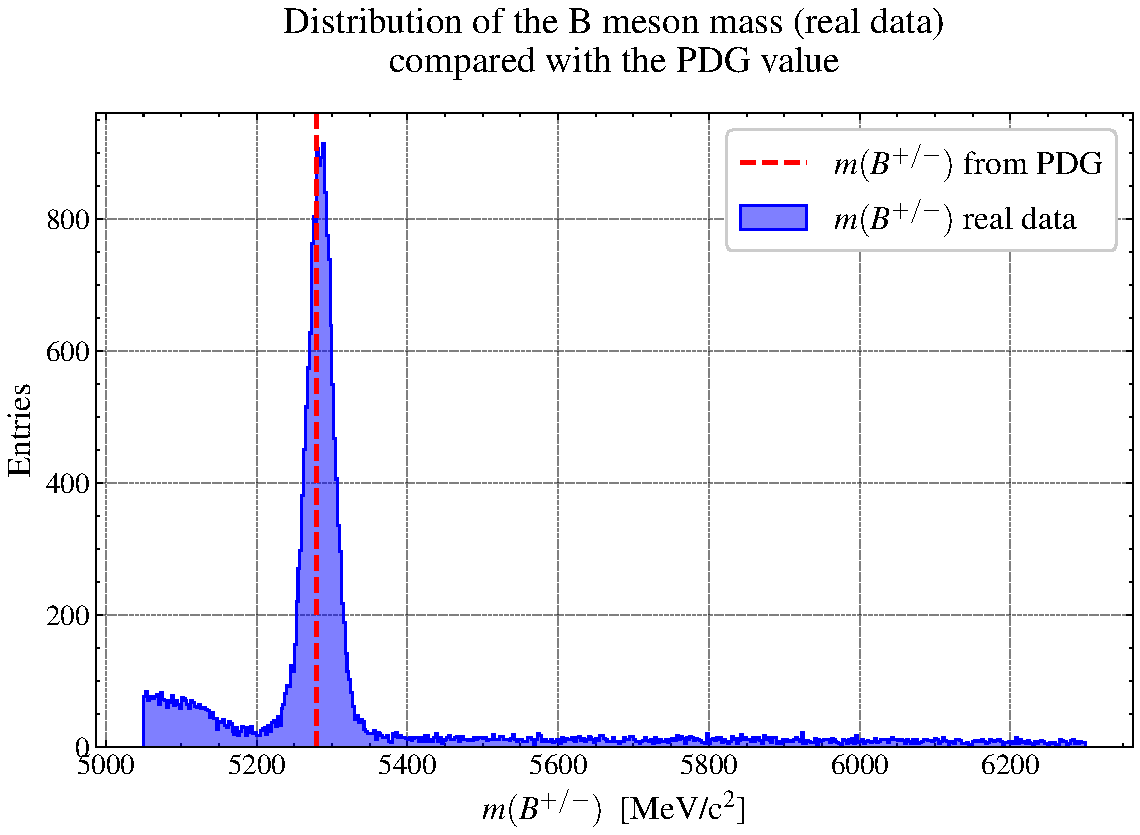
\includegraphics[scale=0.6]{graphs/B_M_data.pdf}}
	\caption{} %caption.}
	\label{fig:B_M_data}
\end{figure}
%-----------------------------------------------------------%

% Global matter anti-matter differences
\subsection{Global CP asymmetry}\label{sec:globCP}

In order to quantify the \emph{global} matter anti-matter asymmetry in this process, we compare the number of $B^{+}$ meson with the number of its anti-particle $B^{-}$.
Computationally, we count the number $N^{+}=12390$ and $N^{-}=11505$ of events with charge $+1$ and $-1$, respectively, in the real dataset\footnote{This measurement can be made more sophisticated and precise: note that in the mass distribution of B mesons there is a peak, called \emph{signal}, and a bottom, called \emph{background}. Therefore, it is possible to refine the selection of events by selecting only the signal, by fitting of the mass distribution to estimate the yield of signal and background events.}.

This allow us to calculate the asymmetry $A_{\mathrm{CP}}$ and the related uncertainty $\sigma_{A}$ and significance $S_{A}$:

\begin{align}
    A_{\mathrm{CP}} &= \frac{N^{+} - N^{-}}{N^{+} + N^{-}}\label{eq:asym} \\[0.5cm]
    \sigma_{\mathrm{CP}}^{A} &= \sqrt{\frac{1 - A_{\mathrm{CP}}^{2}}{N^{+} + N^{-}}}\label{eq:unce} \\[0.5cm]
    S_{\mathrm{CP}}^{A} &= \frac{A_{\mathrm{CP}}}{\sigma_{\mathrm{CP}}^{A}}\label{eq:sign}
\end{align}

In particle physics, a value is only considered an observation, if it is at least five standard deviations, $(> 5\sigma)$. While, if it exceeds three sigma $(> 3\sigma)$, it is considered evidence.

The asymmetry is corrected by the underlying production asymmetry $A_{\mathrm{CP, prod}}$, arising from the fact that the particles are produced by proton-proton collisions.
The production asymmetry is approximated with $\approx 1\%$.
The final asymmetry then is calculated by:

\begin{equation}
    A_{\mathrm{CP, global}} = A_{\mathrm{CP}} - A_{\mathrm{prod}} = 0.0270
\end{equation}

and through the \emph{propagation of uncertainty},

\begin{equation}
    \sigma_{\mathrm{CP, global}}^{A} = \sqrt{(\sigma_{\mathrm{CP}}^{A})^2 + (\sigma_{\mathrm{prod}}^{A})^2} = 0.0092 
\end{equation}

which gives the significance:

\begin{equation}
    S_{\mathrm{CP, global}}^{A} = \frac{A_{\mathrm{CP, global}}}{\sigma_{\mathrm{CP, global}}^{A}} = 2.9348
\end{equation}

%-----------------------------------------------------------%

% Dalitz plots and resonances
\subsection{Dalitz plots}

The decay $B^{\pm} \rightarrow h^{\pm} h^{+} h^{-}$ can occur in two distinct ways:

\begin{itemize}
    \item directly through three-body final state;
    \item via an intermediate particle, a \emph{resonance}, through two-body decay.
\end{itemize}

For example, $B^{+} \rightarrow h^{+} h^{+} h^{-}$ can proceed through the decay $B^{+} \rightarrow h^{+} R_{0}$, where $R_{0}$ is a neutral meson resonance which can decay as $R_{0} \rightarrow K^{+} K^{-}$.

An useful tool to identify resonances in the decay is the \emph{Dalitz plot}: a bidimensional plot in the phase space that represents the possible manners in which the products of certain three-body decays can be produced. The axes of the plot are the squares of the invariant masses of two pairs of the decay products.

Notice that the kinematics of a three-body decay can be fully described using only these two variables (invariant masses of pairs of decay products), since energies and momenta of the three kaons are not independent of each other as they all come from the decay of a B meson and energy and momentum are conserved.

The simulated data do not include resonances and are therefore uniformly distributed, as can be seen in \autoref{fig:dalitz_sim} and \autoref{fig:hist2d_sim}.

\begin{multicols}{2}
    \begin{figure}[H]
        %\setkeys{Gin}{draft=false}
    	\centering
    	\fcolorbox{black}{white}{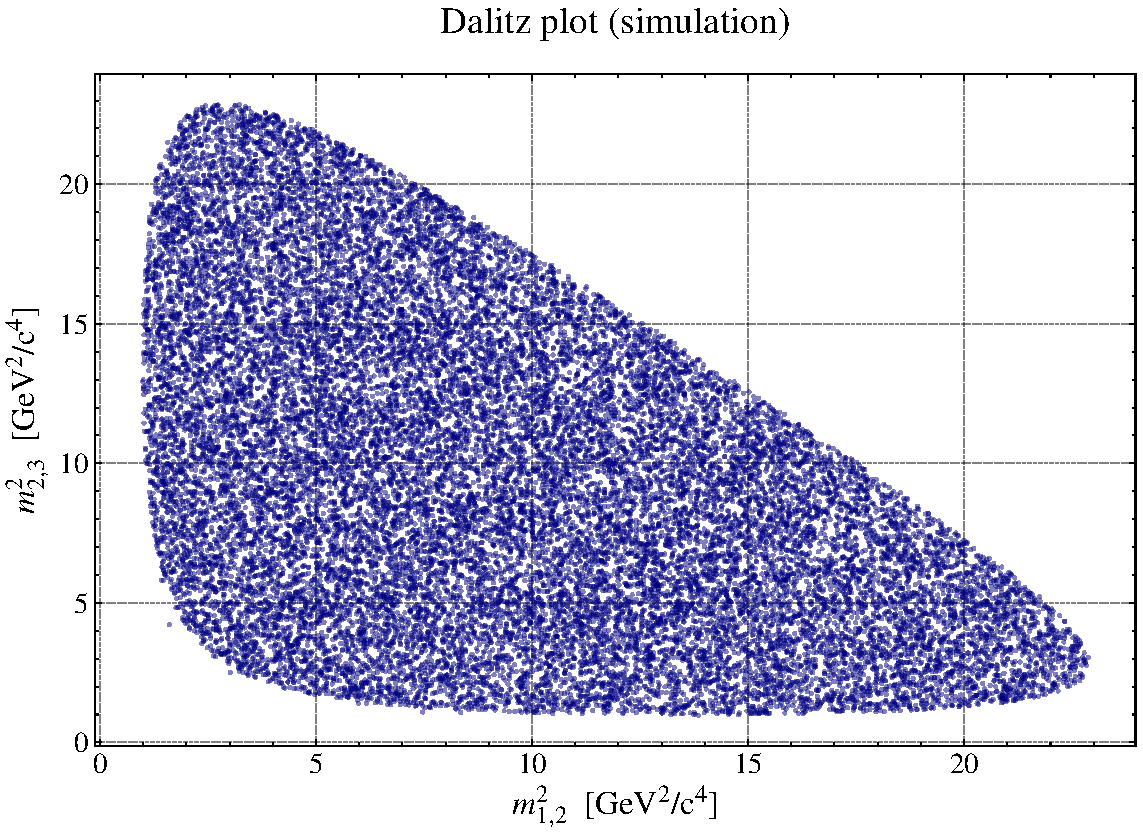
\includegraphics[scale=0.3]{graphs/dalitz_sim.pdf}}
    	\caption{Scatter Dalitz plot of the simulated data.} %caption.}
    	\label{fig:dalitz_sim}
    \end{figure}

    \begin{figure}[H]
        %\setkeys{Gin}{draft=false}
    	\centering
    	\fcolorbox{black}{white}{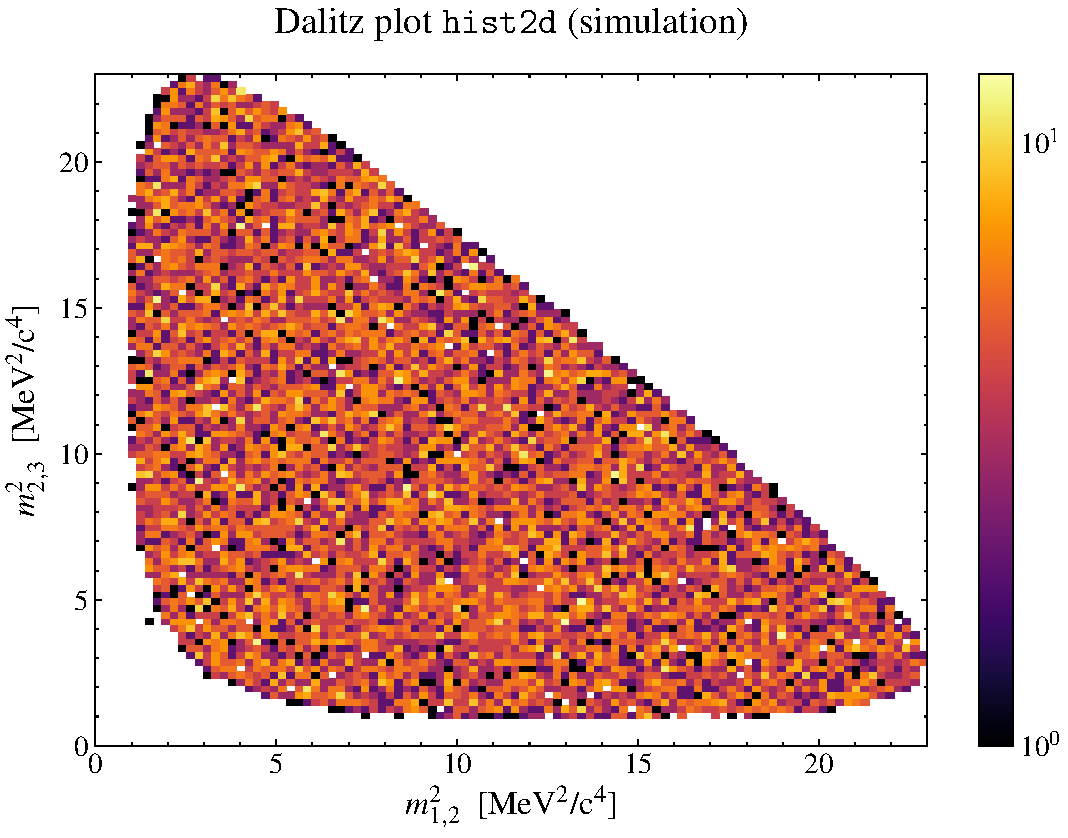
\includegraphics[scale=0.3]{graphs/hist2d_sim.pdf}}
    	\caption{Binned Dalitz plot of the simulated data.} %caption.}
    	\label{fig:hist2d_sim}
    \end{figure}

    \begin{figure}[H]
        %\setkeys{Gin}{draft=false}
    	\centering
    	\fcolorbox{black}{white}{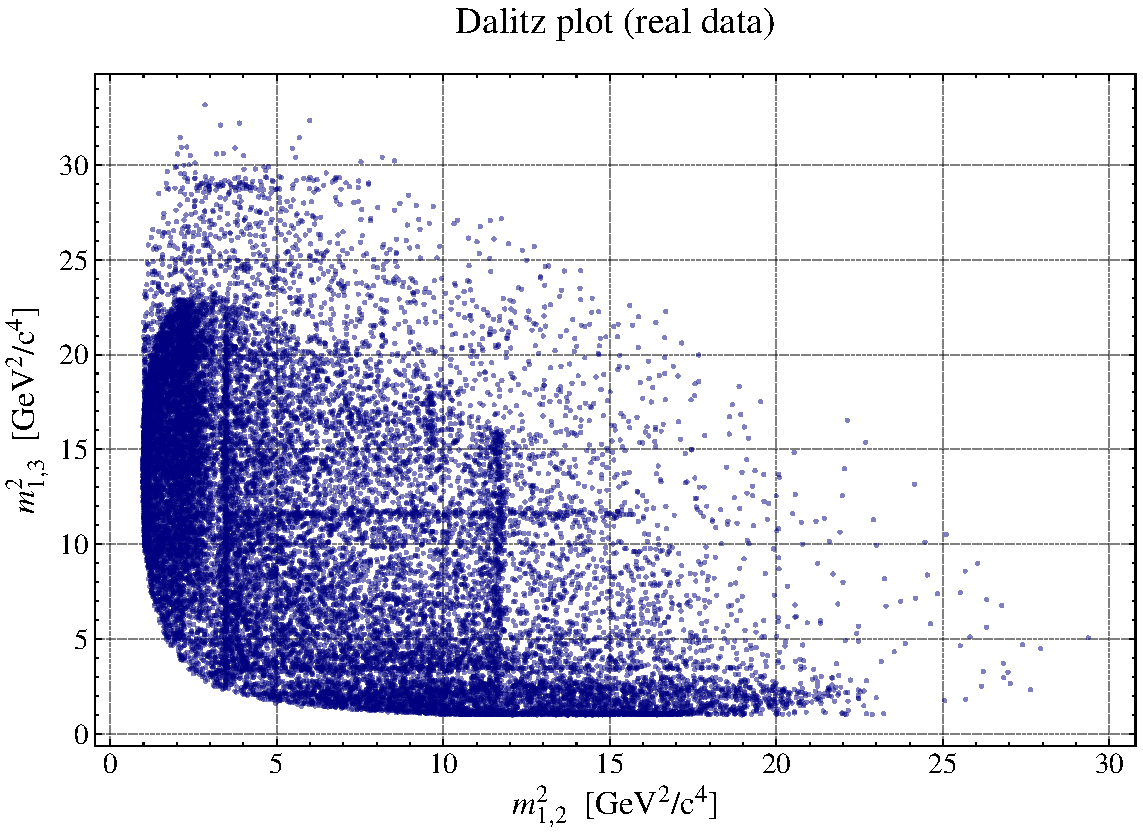
\includegraphics[scale=0.3]{graphs/dalitz_real.pdf}}
    	\caption{Scatter Dalitz plot of the real data.} %caption.}
    	\label{fig:dalitz_real}
    \end{figure}

    \begin{figure}[H]
        %\setkeys{Gin}{draft=false}
    	\centering
    	\fcolorbox{black}{white}{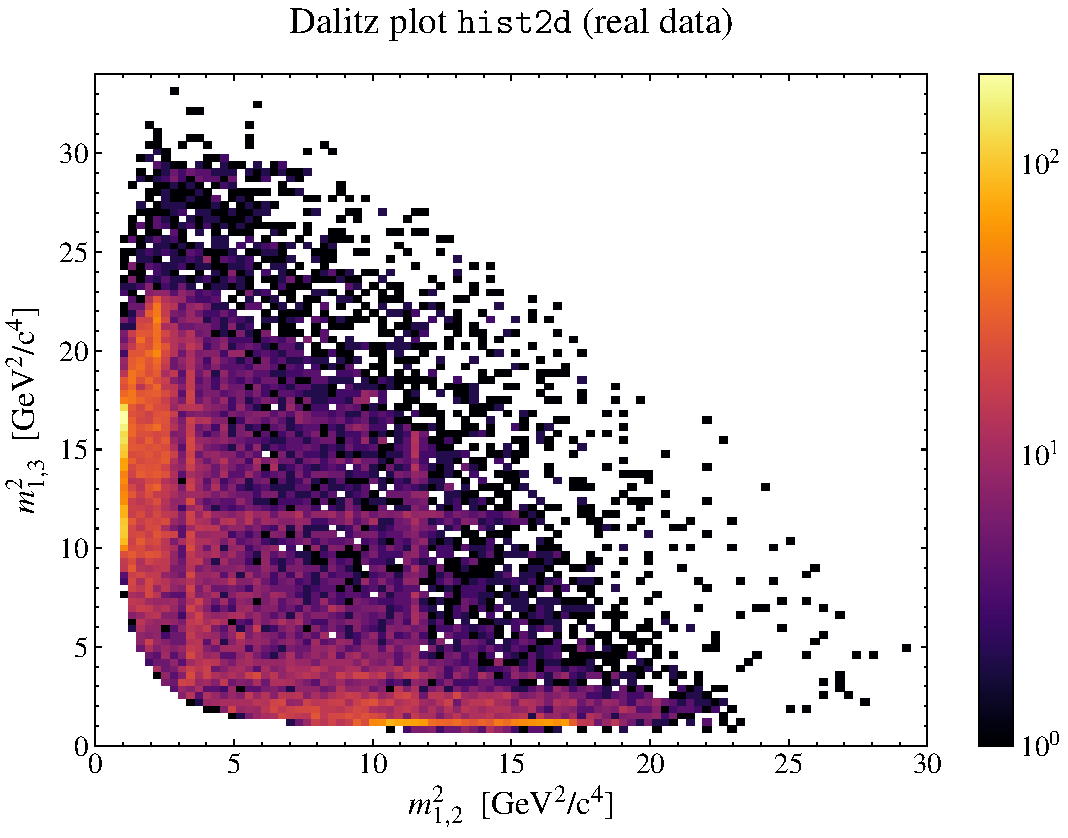
\includegraphics[scale=0.3]{graphs/hist2d_real.pdf}}
    	\caption{Binned Dalitz plot of the real data.} %caption.}
    	\label{fig:hist2d_real}
    \end{figure}
\end{multicols}

While in the real data, since two kaons always have the same charge, there are two possible resonance combinations.
It is important to first look up which kaon candidates are oppositely charged: in our data the second and third kaon candidates have the same charge. Therefore the only possible combinations are $R_{1,2}^0$ and $R_{1,3}^0$.
The $R_{2,3}^0$ combination would result in a charged resonance (with charge: $+2$ or $-2$), which is not provided for in the Standard Model.

So, choosing the invariant masses of $R_{1,2}^0$ and $R_{1,3}^0$ resonances as axes of the Dalitz plot, we are able to identify resonances band structures, visible in \autoref{fig:dalitz_real} and \autoref{fig:hist2d_real}.

%-----------------------------------------------------------%

\subsection{Mass ordered Dalitz plot}

\begin{multicols}{2}
    \begin{figure}[H]
        %\setkeys{Gin}{draft=false}
    	\centering
    	\fcolorbox{black}{white}{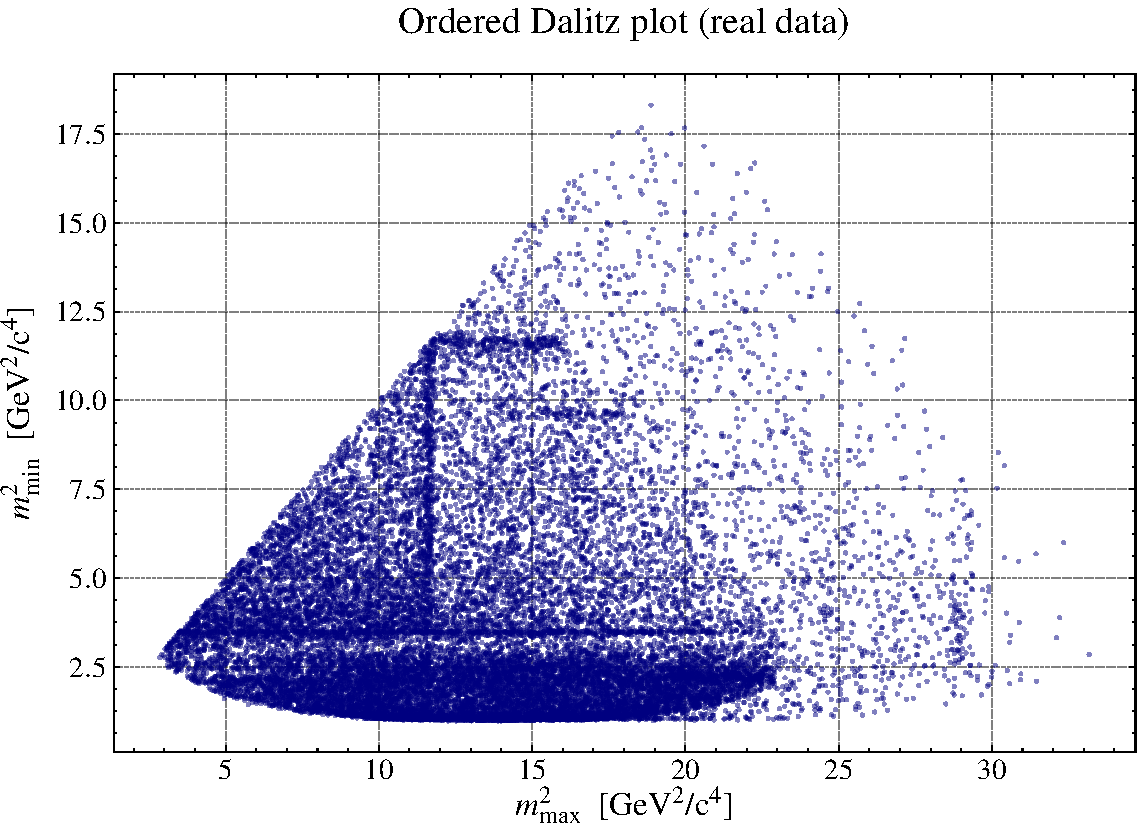
\includegraphics[scale=0.3]{graphs/dalitz_ordered.pdf}}
    	\caption{} %caption.}
    	%\label{fig:enter-label}
    \end{figure}

    \begin{figure}[H]
        %\setkeys{Gin}{draft=false}
    	\centering
    	\fcolorbox{black}{white}{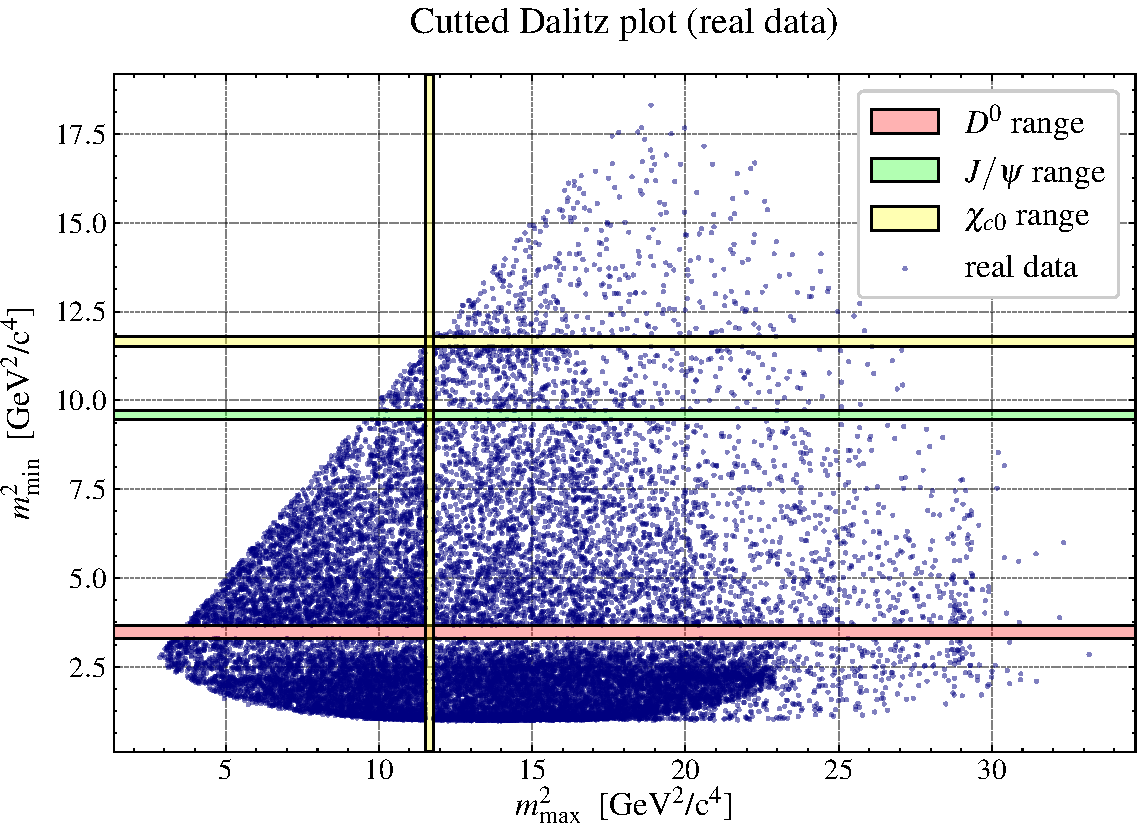
\includegraphics[scale=0.3]{graphs/dalitz_cutted.pdf}}
    	\caption{} %caption.}
    	\label{fig:dalitz_cut}
    \end{figure}

    \begin{figure}[H]
        %\setkeys{Gin}{draft=false}
    	\centering
    	\fcolorbox{black}{white}{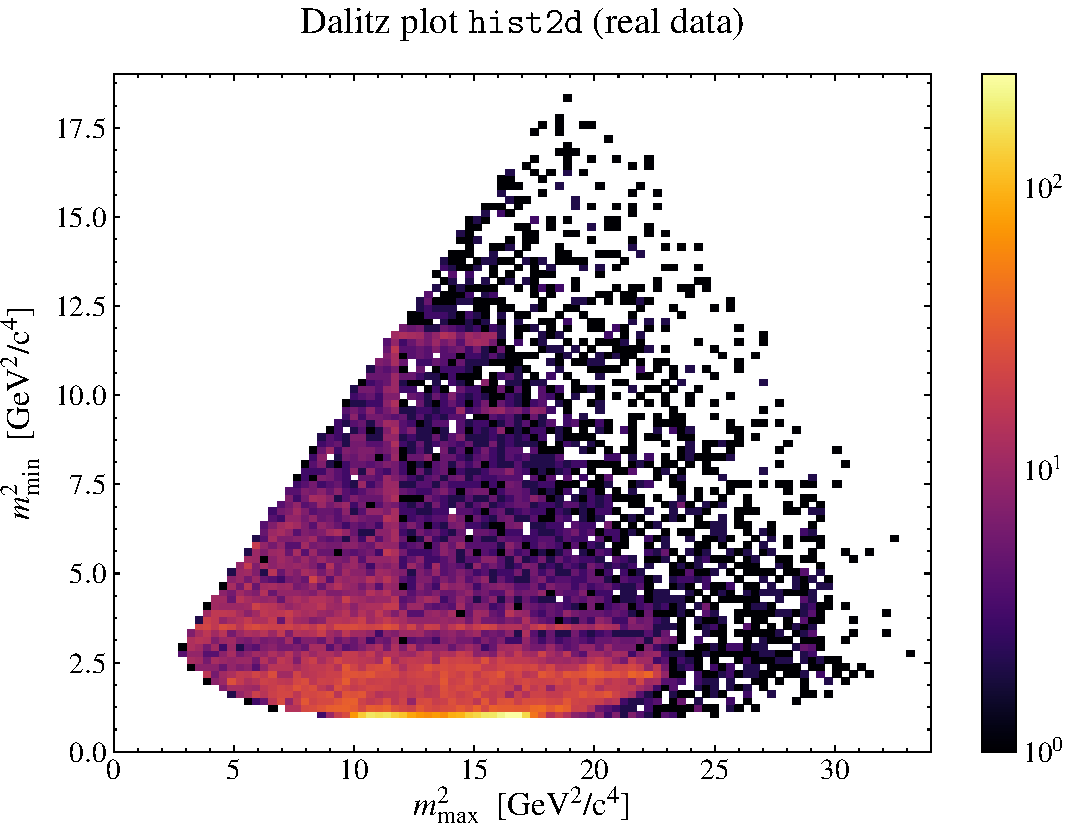
\includegraphics[scale=0.3]{graphs/hist2d_ordered.pdf}}
    	\caption{} %caption.}
    	%\label{fig:enter-label}
    \end{figure}

    \begin{figure}[H]
        %\setkeys{Gin}{draft=false}
    	\centering
    	\fcolorbox{black}{white}{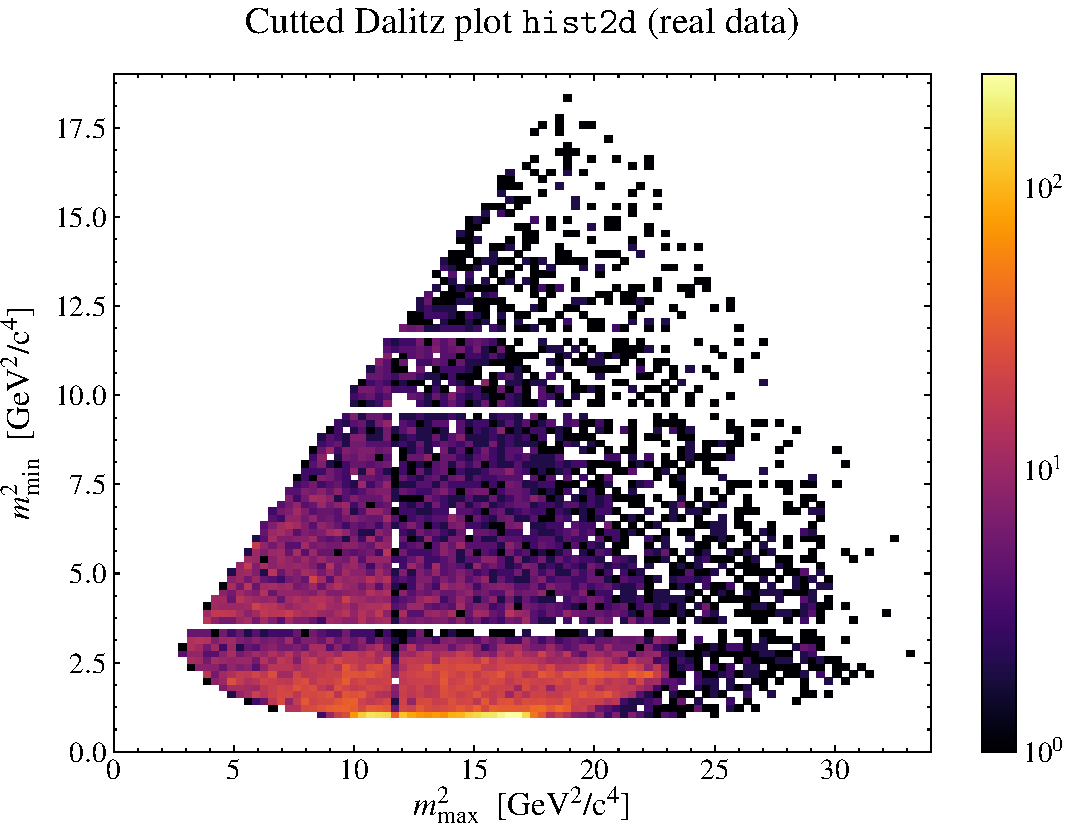
\includegraphics[scale=0.3]{graphs/hist2d_cutted.pdf}}
    	\caption{} %caption.}
    	\label{fig:hist2d_cut}
    \end{figure}
\end{multicols}

To improve the visibility of the resonances in the Dalitz plot it is useful to impose an ordering, so we sort the two resonances in a combination of kaons with the respectively higher mass $R_{\mathrm{max}^{0}}$ and one with the corresponding lower mass $R_{\mathrm{min}^{0}}$.

We now use the mass of these ordered resonances as Dalitz plot variables, thus effectively \enquote{folding} the Dalitz plot, so that one axis always has a higher value than the other. The total energy range is indeed reduced, while still remaining with the same statistics. This leads to a
higher event density and therefore much \enquote{clearer} structures in the Dalitz plots. 

The knowledge of resonances is of fundamental importance because it allows us to exclude from the analysis of the different possible ways in which the three-body decay can occur, those in which we are not interested: in particular, we are studying \enquote{charmless} decays and so we must remove all those resonances in which charm quarks are contained.

We can identify three of this resonances (from the \href{https://pdglive.lbl.gov/Viewer.action}{PDG} \cite{PDG}):

\begin{itemize}
    \item $m(D^{0}) = 1864.84 \pm 0.05$ [MeV/c$^2$]
    \item $m(J/\Psi) = 3096.900 \pm 0.006$ [MeV/c$^2$]
    \item $m(\chi_{c0}) = 3414.71 \pm 0.30$ [MeV/c$^2$]
\end{itemize}

that we remove, using the following cut: 

\begin{lstlisting}
D^0 range:   [ 3.3 -  3.7] [GeV^2/c^4]
JPSI range:  [ 9.5 -  9.7] [GeV^2/c^4]
CHIc0 range: [11.5 - 11.8] [GeV^2/c^4]
\end{lstlisting}

This result in the Dalitz plot without resonances as in \autoref{fig:dalitz_cut} and \autoref{fig:hist2d_cut}.
%-----------------------------------------------------------%

% Local matter anti-matter differences
\subsection{Local CP asymmetry}

Previously, (\Cref{sec:globCP}), we calculated the global CP asymmetry, but the asymmetry value obtained was not that much significant ($<3\sigma$). To improve this result and obtain a higher significance value, we try to calculate the \emph{local} CP asymmetry.
Indeed CP violation arises from interference between different decay chains with different intermediate resonances to a common final state. Therefore, the strength and the sign of the CP violation might vary in different kinematic regions.

For this reason, we are interested in identify those kinematic regions where CP asymmetry is maximized. Therefore, we produce two separate Dalitz plot each for $B^{+}$ and $B^{-}$ decays and we look for asymmetries between those plots, as a signature of CP violation.
Basically, we use $\texttt{hist2d}$ plots to split the events in different bins and count the amount of events for each bin: in order that the statistical error on the asymmetry in each bin is not overly large, the bins need to contain a reasonable number of entries. We use a bin area of $4.6143$ [GeV$^2$/c$^4$].

In \autoref{fig:dalitz_Bplus} and \autoref{fig:hist2d_Bplus} there are the Dalitz and $\texttt{hist2d}$ plots for the $B^{+}$, while in \autoref{fig:dalitz_Bminus} and \autoref{fig:hist2d_Bminus} for the $B^{-}$.  

\begin{multicols}{2}
    \begin{figure}[H]
        %\setkeys{Gin}{draft=false}
    	\centering
    	\fcolorbox{black}{white}{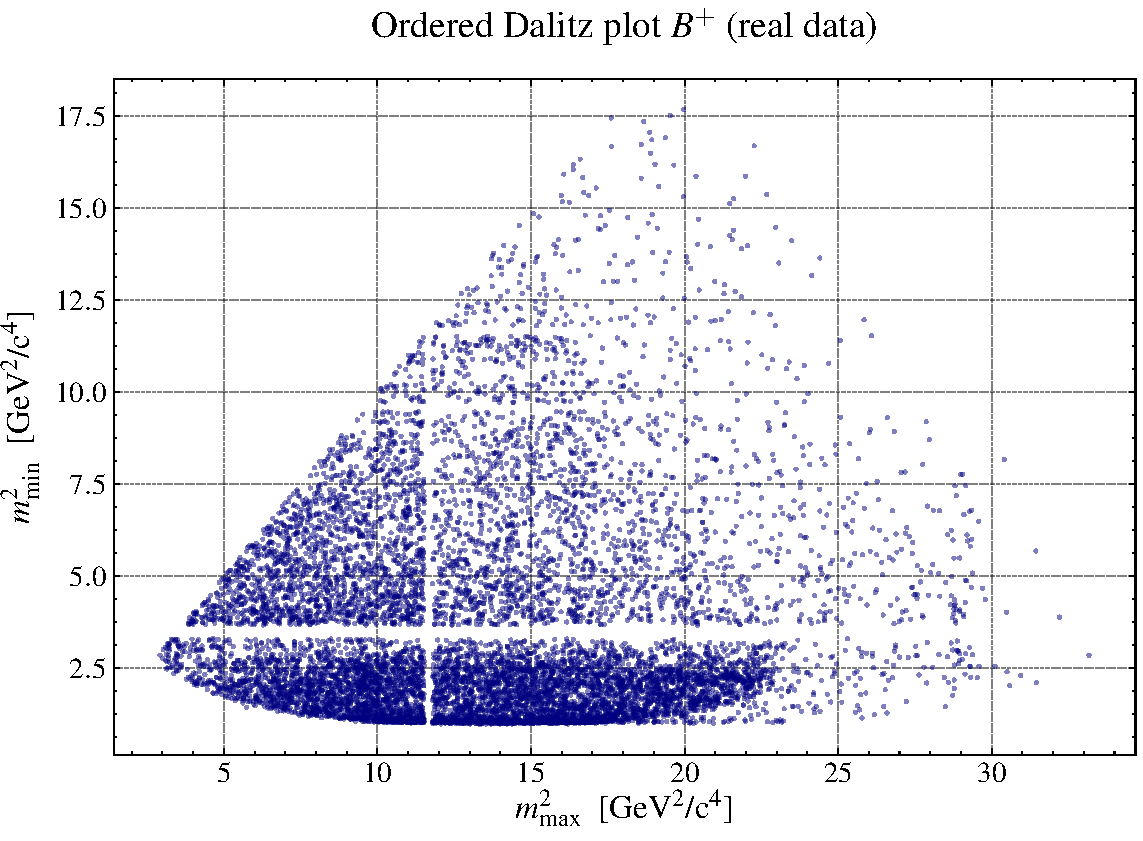
\includegraphics[scale=0.3]{graphs/dalitz_orderedBplus.pdf}}
    	\caption{} %caption.}
    	\label{fig:dalitz_Bplus}
    \end{figure}

    \begin{figure}[H]
        %\setkeys{Gin}{draft=false}
    	\centering
    	\fcolorbox{black}{white}{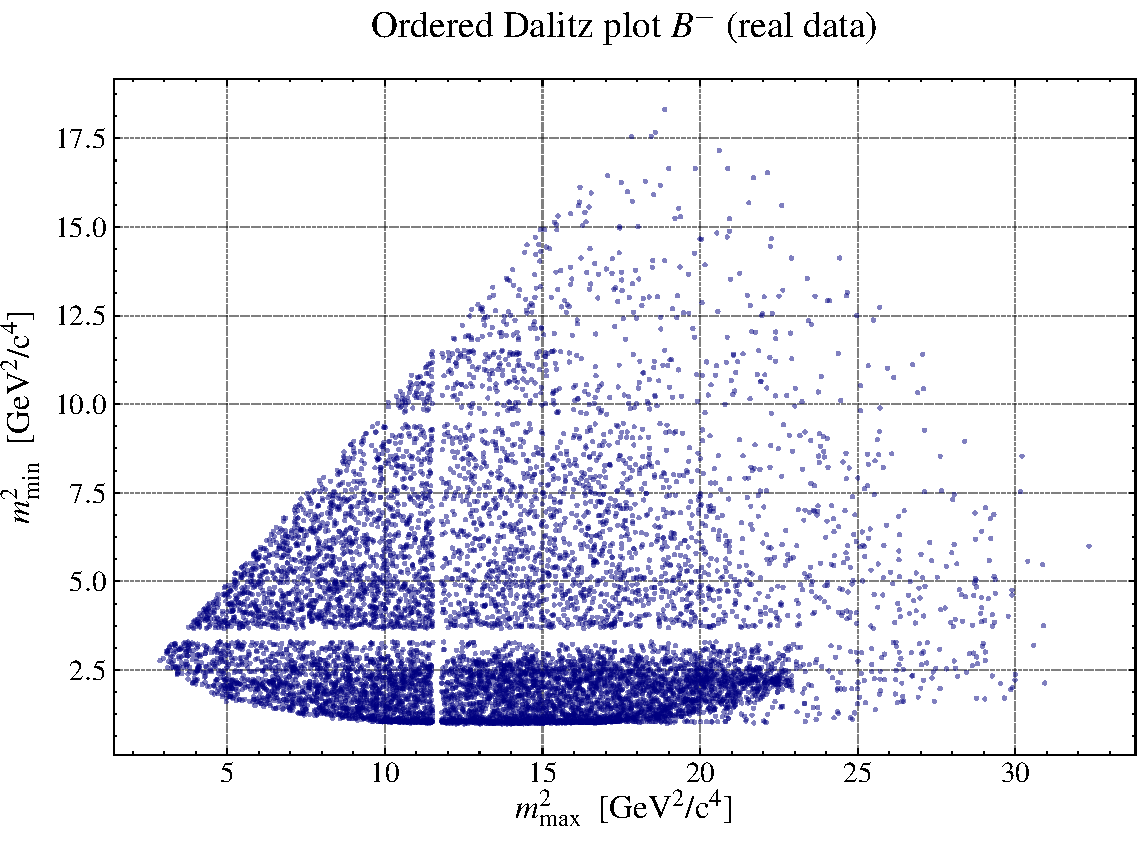
\includegraphics[scale=0.3]{graphs/dalitz_orderedBminus.pdf}}
    	\caption{} %caption.}
    	\label{fig:dalitz_Bminus}
    \end{figure}

    \begin{figure}[H]
        %\setkeys{Gin}{draft=false}
    	\centering
    	\fcolorbox{black}{white}{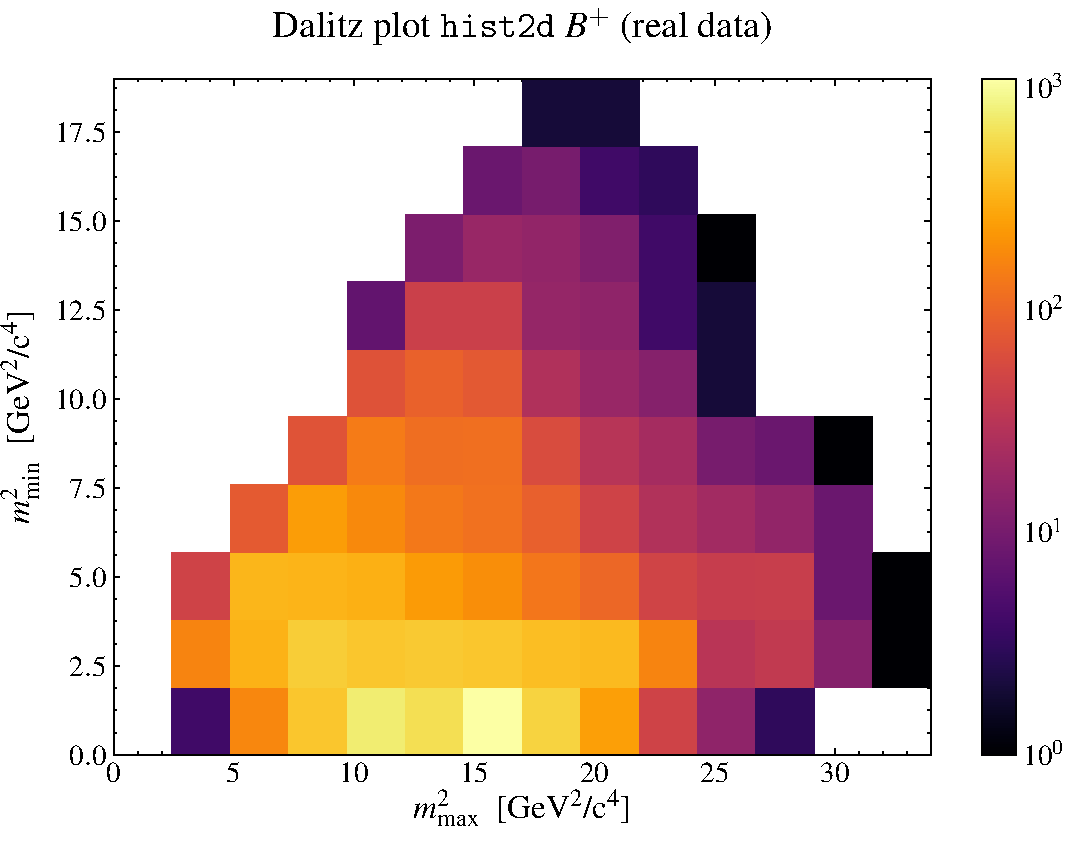
\includegraphics[scale=0.3]{graphs/hist2d_orderedBplus.pdf}}
    	\caption{} %caption.}
    	\label{fig:hist2d_Bplus}
    \end{figure}

    \begin{figure}[H]
        %\setkeys{Gin}{draft=false}
    	\centering
    	\fcolorbox{black}{white}{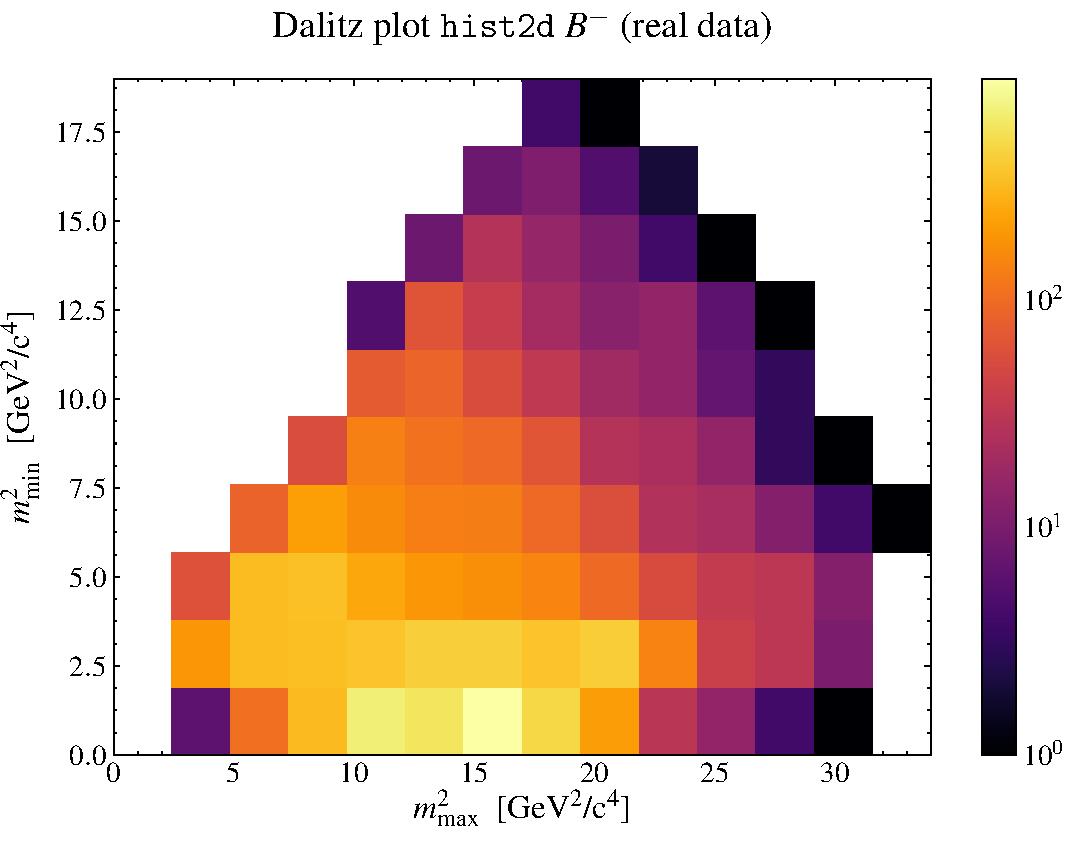
\includegraphics[scale=0.3]{graphs/hist2d_orderedBminus.pdf}}
    	\caption{} %caption.}
    	\label{fig:hist2d_Bminus}
    \end{figure}
\end{multicols}

Since we used the same binning for both $\texttt{hist2d}$ plots, we can calculate the CP asymmetry, $A_{\mathrm{CP}}$, for each bin, comparing the number of events per bin of $B^{+}$ and $B^{-}$, and applying \autoref{eq:asym}. The result is shown in \autoref{fig:hist2d_asym}. We have to pay attention and remember that observing a large asymmetry in some kinematic regions of the plot does not necessarily mean we have CP violation: if there are only very few events in that region of the plot the uncertainty on that large asymmetry may be large, too. Hence, the value may still be compatible with zero.

Therefore, we need to compute the uncertainty
$\sigma_{\mathrm{CP}}^{A}$ and the significance
$S_{\mathrm{CP}}^{A}$ \emph{per bin}, as we have already done in \Cref{sec:globCP} with \autoref{eq:sign} and \autoref{eq:sign}.

This procedure allow us to identify the bins with highest significance (the three marked in red in \autoref{fig:hist2d_signif}), with the following values of significance:

\newpage
\begin{lstlisting}
s.T[0,2] = 3.9444
s.T[0,3] = 4.1711
s.T[1,3] = 4.7866
\end{lstlisting}

The total number of (positive and negative charged) events in this selected kinematic range is $N^{+}=1066$ and $N^{-}=756$.

So we can compute the local CP asymmetry, $A_{\mathrm{CP, local}}$, in this range and consequently the local uncertainty
$\sigma_{\mathrm{CP, local}}^{A}$ and the local significance
$S_{\mathrm{CP, local}}^{A}$.

(The computed values are corrected by the production asymmetry $A_{\mathrm{prod}}$, as in \Cref{sec:globCP}).

\begin{alignat}{2}
    A_{\mathrm{CP, local}} &= A_{\mathrm{CP}} - A_{\mathrm{prod}} &&= 0.1601 \\[0.5cm]
    \sigma_{\mathrm{CP, local}}^{A} &= \sqrt{(\sigma_{\mathrm{CP}}^{A})^2 + (\sigma_{\mathrm{prod}}^{A})^2} &&= 0.0329 \\[0.5cm]
    S_{\mathrm{CP, local}}^{A} &= \frac{A_{\mathrm{CP, local}}}{\sigma_{\mathrm{CP, local}}^{A}} &&= 4.8663
\end{alignat}

\begin{multicols}{2}
    \begin{figure}[H]
        %\setkeys{Gin}{draft=false}
    	\centering
    	\fcolorbox{black}{white}{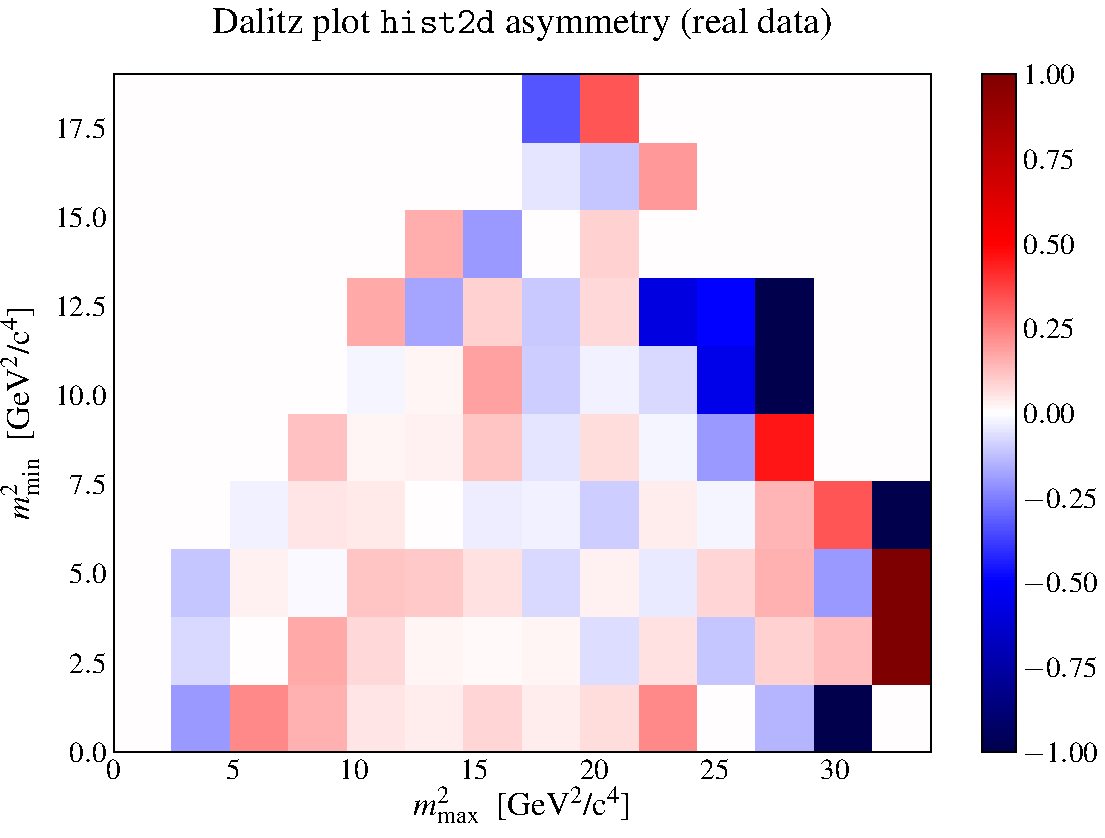
\includegraphics[scale=0.3]{graphs/hist2d_asymmetry.pdf}}
    	\caption{} %caption.}
    	\label{fig:hist2d_asym}
    \end{figure}

    \begin{figure}[H]
        %\setkeys{Gin}{draft=false}
    	\centering
    	\fcolorbox{black}{white}{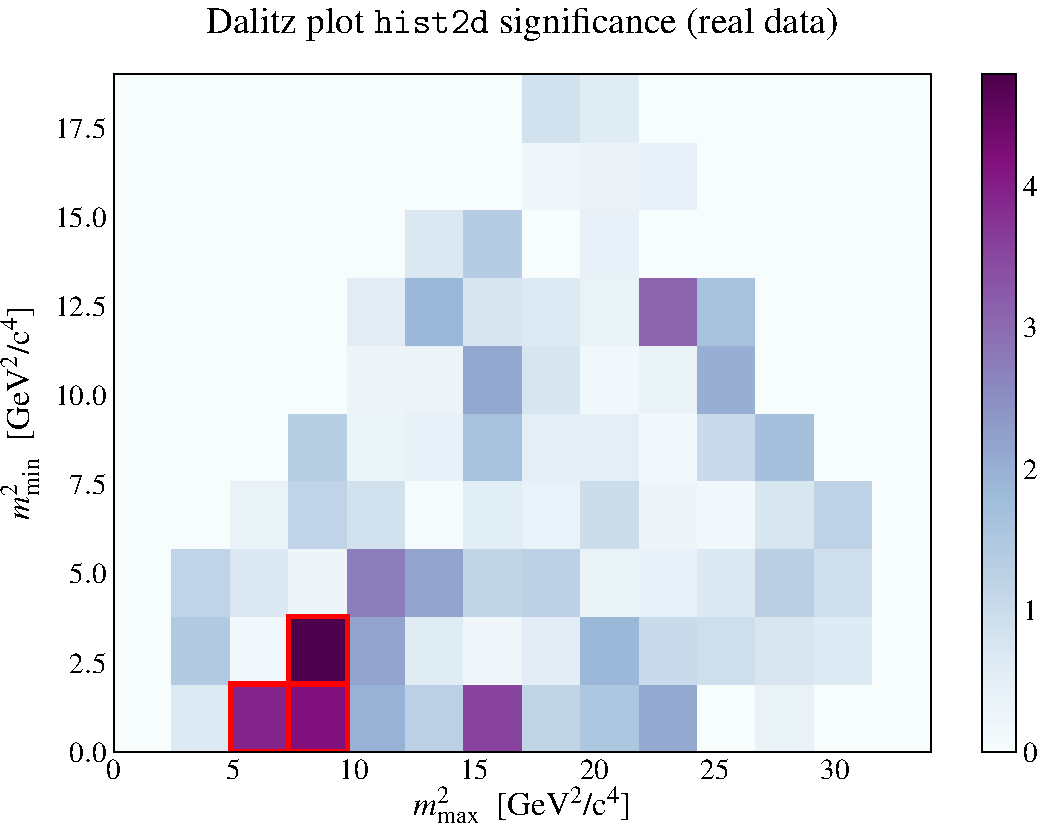
\includegraphics[scale=0.3]{graphs/hist2d_signif.pdf}}
    	\caption{} %caption.}
    	\label{fig:hist2d_signif}
    \end{figure}
\end{multicols}

Finally, we select the $B^{+}$ and $B^{-}$ real data in the maximal CP violation kinematic range and plot the mass distributions, showing the asymmetry visible in the peak, as in \autoref{fig:B_M_asym}:

\begin{figure}[H]
    %\setkeys{Gin}{draft=false}
    \centering
    \fcolorbox{black}{white}{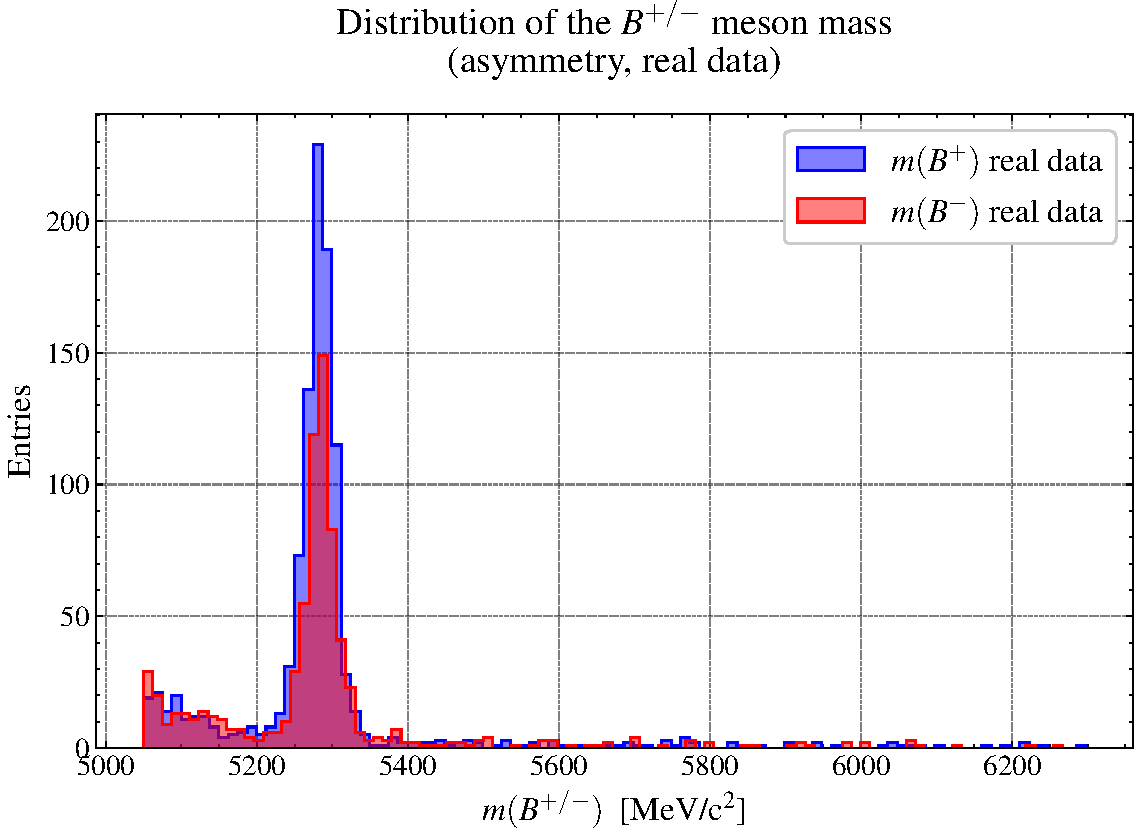
\includegraphics[scale=0.6]{graphs/B_M_asym.pdf}}
    \caption{} %caption.}
    \label{fig:B_M_asym}
\end{figure}

The found local CP asymmetry can therefore be called an \enquote{evidence} of a local CP asymmetry in $B^{\pm} \rightarrow h^{\pm} h^{+} h^{-}$.
%-----------------------------------------------------------%
